\section{What about sets?}%
\label{sec:what_about_sets_}

\begin{frame}
	\frametitle{Sets}
	
	\begin{center}
		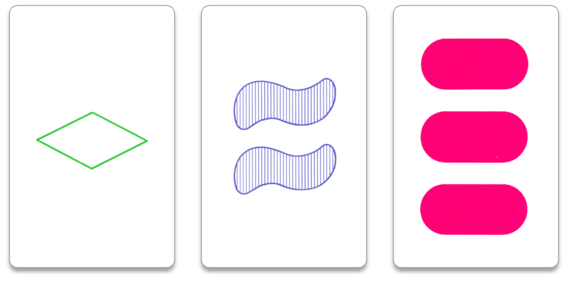
\includegraphics[width=0.8\textwidth]{figures/set.png}\\
		\hspace*{15pt}\hbox{\scriptsize Image By:\thinspace{\itshape MilesK}}
		% https://commons.wikimedia.org/wiki/File:Set-game-cards.png
	\end{center}
\end{frame}

\begin{frame}
	\frametitle{Umm...}

	\begin{questionblock}{What about sets?}
		How can we now implement sets?
	\end{questionblock}
	\pause
	\begin{answerblock}{Valueless things they are\dots}
		A set is just a dict, but without values!	\\
		We call them hashsets, and they are hashmaps without storing values for their keys.\\
		\pause
		So with a good hash function, we can do insertion/deletion and containment-checks in $O(1)$ time.
	\end{answerblock}
\end{frame}
